\section{Simulation Techniques and Physics Scenarios\label{simSetup}}

The simulation of background in the LHC can be very demanding in terms of CPU as detailed shower simulations have to be performed along several hundred meters or many millions of primaries have to be tracked to get sufficient particles leaking to collimators in IR1 or IR5 which by definition is many orders of magnitudes lower than protons hitting the primary collimators. Two simulation codes were used as main tools: SixTrack for particle tracking around the ring and \fluka~for particle showering. 

The layout of nominal LHC is shown in Fig.~\ref{nominalLHC_layout} for intersertion region 1 (IR1) with the interaction point 1 (IP1) at s~=~0. By design, the left and the right side are symmetric for incoming and outgoing beams. For our purposes, shower evaluation from different background sources, it is sufficient to use only half of the layout for the incoming beam. 

%Note, that usually the distributions are indicated per interaction, for beam-halo (BH) simulations distributions are shown per hit in the tertiary collimators and for beam-gas (BG) it is given per proton-nitrogen interaction.

\subsection{Beam-Halo simulations}
The simulation is performed in two steps: First, we use SixTrack~\cite{SixTrackRef} for particle tracking in order to obtain the leakage onto the TCTs in the IRs. To be CPU efficient, only a halo proton distribution is tracked not the full beam with its core that is usually many orders of magnitude more dense. Tracking is performed through a magnetic field lattice, usually prepared using MadX, and the LHC collimatiors of which only the jaws are modeled. We also assume a perfect machine, neglecting any uneven jaw surfaces or edges\footnote{Previous studies REFERENCE have shown if one includes machine errors, the results differ by a factor of about 2.}.

The beam halo is usually simulated in horizontal (h) and vertical (v) distributions, these are flat in one plane and Gaussian in the other (for more information see also~\cite{chiarasThesis}). When a collimator is hit, a built-in, recently updated Monte-Carlo model~\cite{claudiasThesis} decides on the physics process. Protons continue in the lattice until they dissociate in an inelastic interaction with the collimator material or (in a post-processing step) are lost on the aperture. As a result, loss locations around the ring can be identified and protons absorbed by the TCTs serve in second step as seeds in \fluka~\cite{flukaRef1,flukaRef2}~to evaluate particle showers streaming towards the detector. Particle interaction and transport are calculated within matter for a user-defined geometry. It uses modern physics models and experimental data as available by the Particle Data Group~\cite{pdgRef}. The geometry was built up to 546~m of the right side of IR1 for the present LHC machine, for HL-LHC scenarios the geometry reaches up the tertiary collimators of around 215~m including the long straight section of IR1 (LSS1).

When halo protons interact with the jaw material of the TCTH or TCTV shower particles are created and stream towards the experiment. Every particle passing an imaginary (x,y)-plane at 22.6~m away from the IP, essentially between the triplet magnets and the TAS, is recorded and written out. The left plot of Fig.~\ref{tctHits} shows part of the \fluka~geometry and in green the hits in an horizontal collimator TCTH.4L1 with absorbed protons from an horizontal and vertical halo distribution. On the right of Fig.~\ref{tctHits} one can see how deep these positions are with respect to the jaw surface shown for the collimator pair of IR1. This depth distribution is shown here as an example, but we can note that the shallower the distribution is, the more of the created shower is not confined and contributes to background at the interface plane.

\begin{figure}%[!htb]
\begin{center}
\includegraphics[width=0.9\textwidth]{figures/IR1_layout_runII.pdf}
\end{center}
\vspace{-0.6cm}
 \caption{Machine layout for the nominal LHC (as in Run I and II) of the left side of IR1 with IP1 at s = 0 for the incoming beam. Highlighted are the tertiary collimators (TCT4) at around -147~m, TCLs are debris collimators for the outgoing beam.
  \label{nominalLHC_layout}}
\end{figure}


%% \begin{figure}
%% \begin{center}
%% 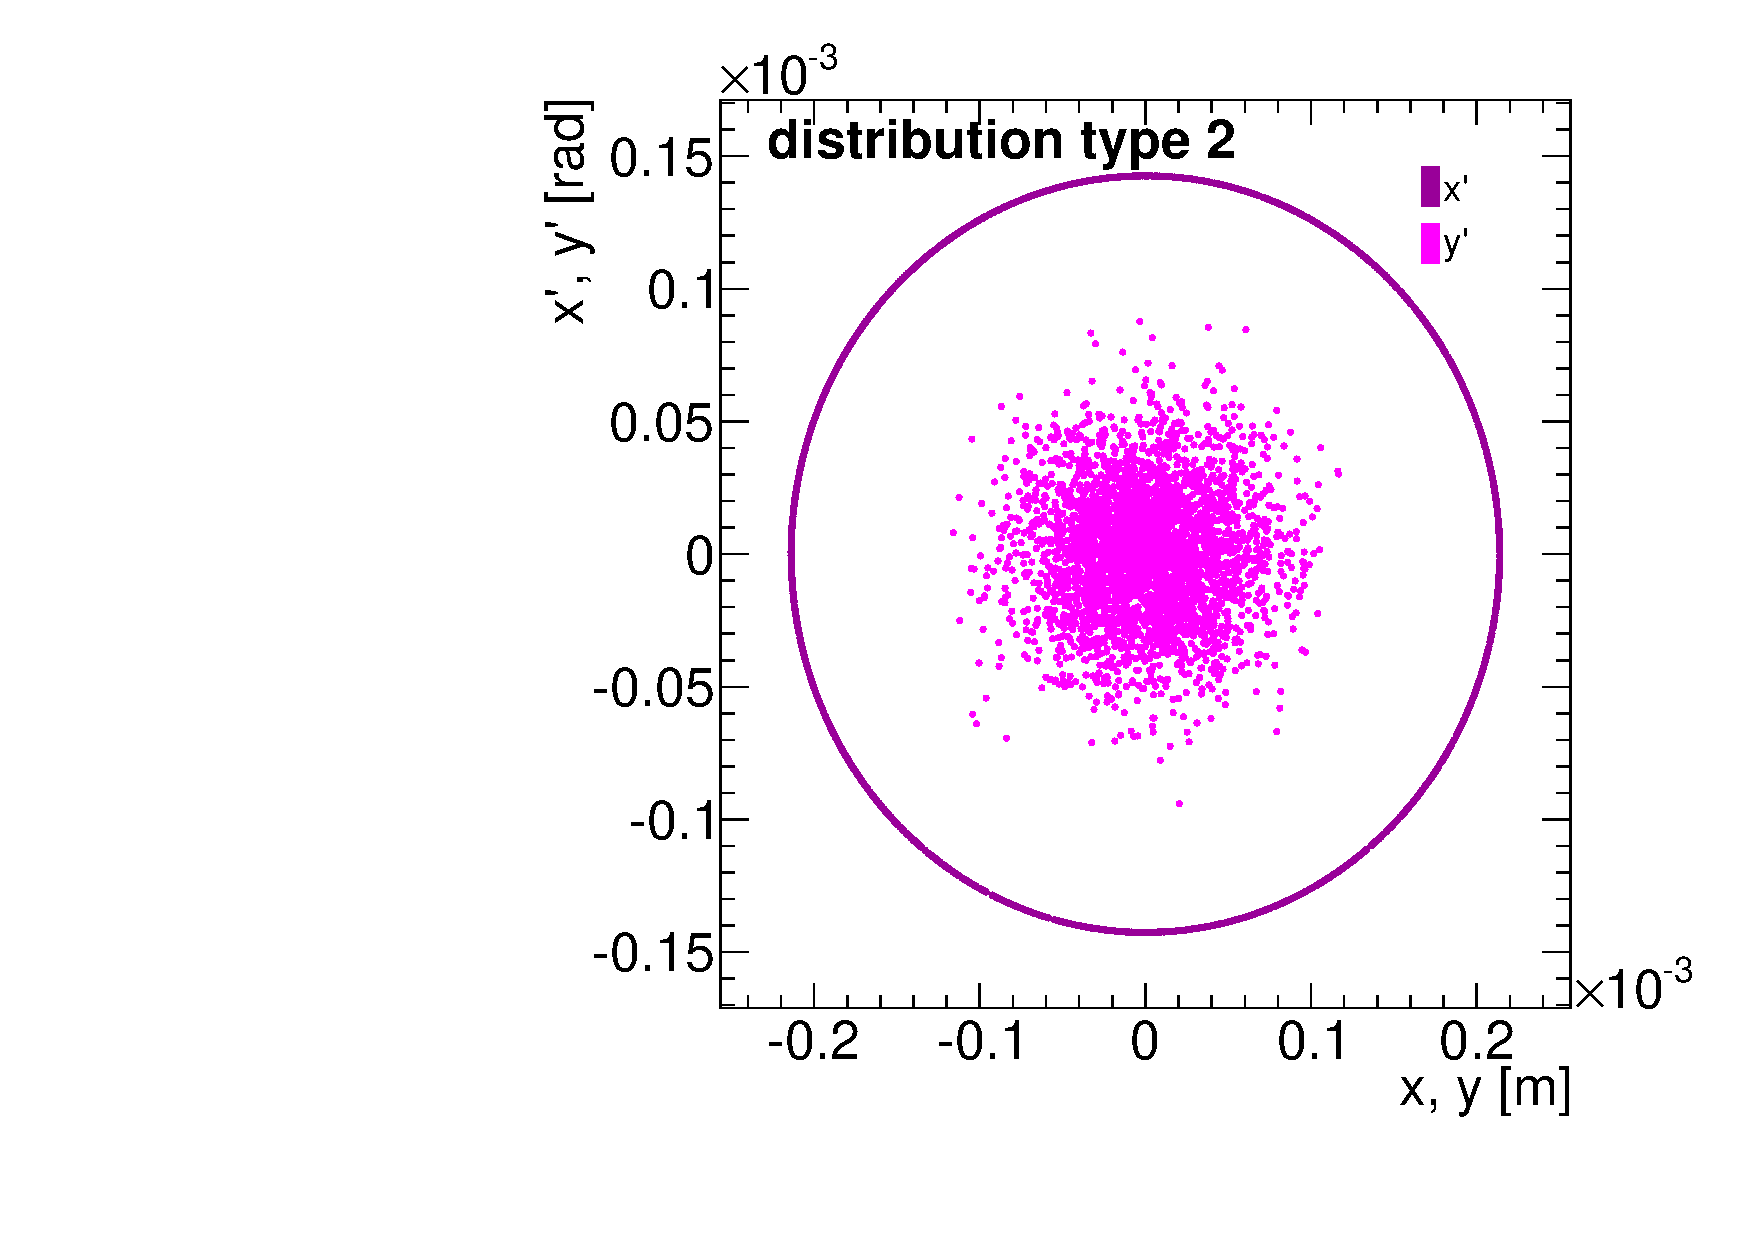
\includegraphics[width=0.48\textwidth]{figures/phasespace_d2}
%% 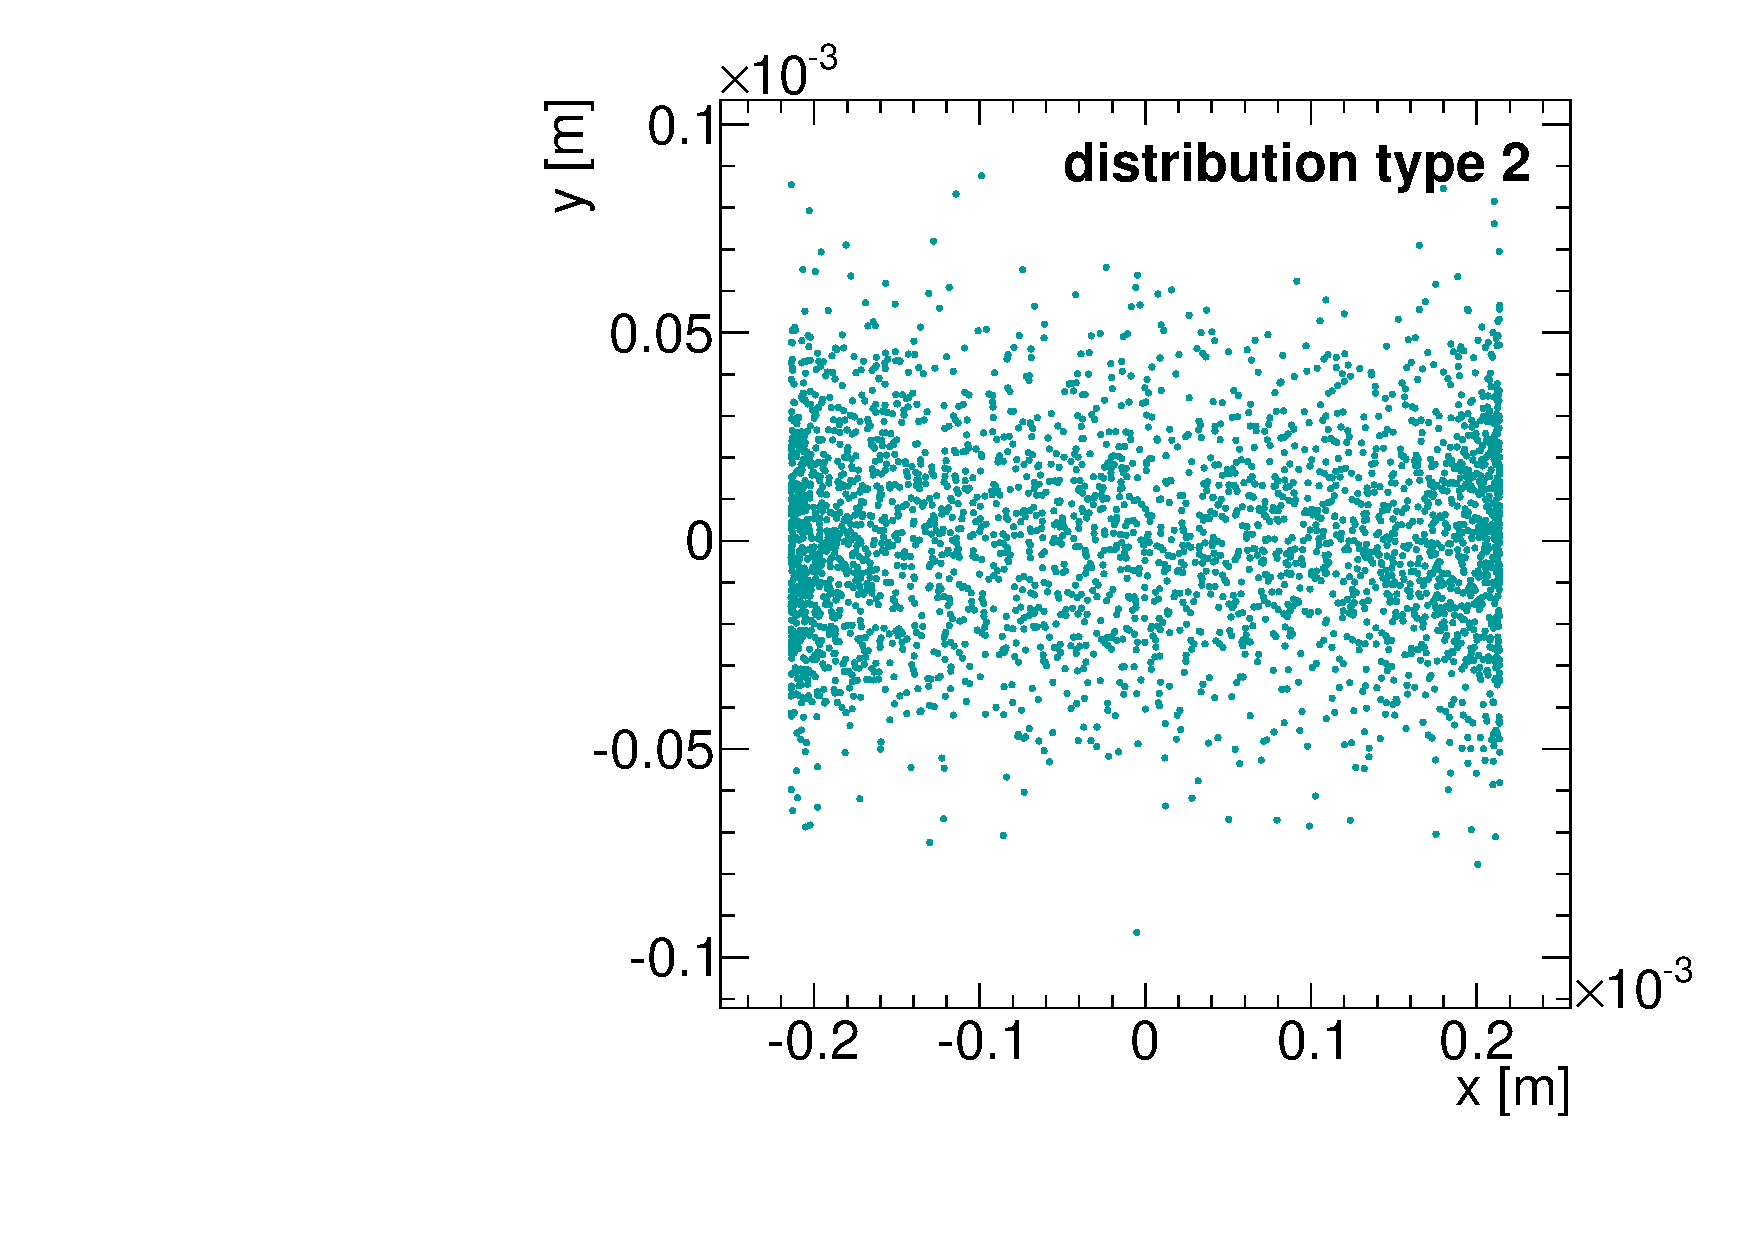
\includegraphics[width=0.48\textwidth]{figures/realspace_d2}
%% \end{center}
%% \caption{Initial halo distribution of type 2 in phase-space (left) and real space (right) is generally used in horizontal halo simulations with SixTrack.
%% \label{haloExamples}}
%% \end{figure}


\begin{figure}%[!htb]
\begin{center}
\includegraphics[width=0.9\textwidth]{figures/IR1_interfaceplane.pdf}
\end{center}
\vspace{-0.6cm}
 \caption{x-z cut of \fluka~geometry zoomed into the interface region between detector and machine. A virtual plane at 22.6 m is used to evaluate particle showers. Each color defines a different material.
  \label{flukaGeo_nominal}}
\end{figure}


\begin{figure}%[!htb]
\begin{center}
  \includegraphics[width=0.4\textwidth]{figures/6500GeV/xz_6500GeV_b1_TCT4.pdf}
  \includegraphics[width=0.4\textwidth]{figures/6500GeV/inelposition_sum_HALOB1.pdf}
\end{center}
\vspace{-0.6cm}
 \caption{View in the (x,z)-plane of hits in TCTH from the Run~II halo simulation case zoomed into the inner collimator parts. The hits are all contained within the collimator jaws and were obtained by SixTrack and transformed to the positions of the TCT in the \fluka~coordinates.
  \label{tctHits}}
\end{figure}


\subsection{Beam-Gas simulations}

We simulate local beam-gas interactions in a \fluka~geometry up to $s$ = 546.6~m of IR1. Inelastic proton-nitrogen interactions are uniformly sampled all along $s$ and these positions used to be on the ideal orbit of the beam trajectory. We introduced a new way of sampling taking into account the transverse expansion of the beam which is described in detail further below.
Like for the beam-halo simulations, information of each shower particle reaching the virtual interface plane at 22.6~m is recorded.

In \fluka, inelastic interactions were sampled uniformly from certain positions. If one has a non-flat pressure profile, one can either reweight at run-time or in a subsequent step if one keeps the information of the initial s-position of the interacting proton of each particle at the interface plane. The advantage of the second method is that distributions can be easily re-normalised to another pressure profile. For earlier simulations, as performed for beam-gas studies in an HL-LHC scenario~\cite{ipac2014_rkh}, this functionality was not in place, however the normalisation for studies shown here were all done in a sub-sequent step. In both simulation cases, beam-gas in Run~I (2012) and Run~II (2015), nitrogen was chosen as collision partner of the beam proton in the simulations as the measured pressures are calibrated against nitrogen and given in nitrogen equivalent.

\begin{table}
   \centering
   \caption{Inelastic atomic cross-sections for the rest gas and LHC beam protons with the main gas species being H$_2$, CH$_4$, CO and CO$_2$. Extracted from \fluka.}
   \begin{tabular}{c|c|c}

       $\sigma$ [mb] & E$_{beam}$ = 4 TeV   & E$_{beam} =$ 6.5 TeV \\ \hline\hline
       H & 37.1 & 38.4 \\
       C & 260& 269 \\
       O & 318 & 329 \\

   \end{tabular}
   \label{tab:atomicXsections}
\end{table}

The inelastic cross-sections are listed in Tab.~\ref{tab:atomicXsections} and were extracted from \fluka. Note that in \fluka, the cross-sections are indicated as an interaction probability per unit length per atom (macroscopic cross-section), e.g.~[$\sigma^{\textrm{macro}}$] = $\frac{1}{cm}$. To convert to the microscopic cross-section, this formula was used: $\sigma^{\textrm{micro}} = \frac{N_A \cdot A \cdot \sigma^{\textrm{macro}}}{\rho}$ with $N_A$ the Avogadro constant [$\frac{g}{mol}$], $A$ the atomic weight [$mol$] and $\rho$ the density of the atom [$\frac{g}{cm^3}$].

These were used to compute rate of the interaction probability of a specific gas $i$ per beam proton which is the product of the number of available gas molecules (or atoms), given be the density $\rho_i$ of that species, and its cross-section $\sigma_i$ divided by the revolution period of the beam $T_{\mathrm{rev}}$:
\begin{equation} \label{eq2}
p_{\mathrm{int},i} = \sigma_{i} \cdot \rho_{i}(s) \cdot \frac{1}{T_{\mathrm{rev}}}
\end{equation}

The reweighting method is the same as in Ref.~\cite{nimPaperRod}. We write down the calculation of weights for each bin $j$ as applied to the bin content of bin $j$ that is already in a binning-independent representation and normalised to the total number of simulated beam-gas interactions 

\begin{equation} \label{eq3}
\mathrm{weight}_j = N_{\mathrm{protons}} \cdot p_{\mathrm{int}}^{\mathrm{tot}} (s_j) \cdot \Delta s_{j} 
\end{equation}

with the total rate of interaction probabilities of each atom $i$ at the position $s_j$ 
\begin{equation*} 
  p_{\mathrm{int}}^{\mathrm{tot}} (s_j) = \Sigma_i \, p_{\textrm{int},i}
\end{equation*}

and the length $\Delta s_{j}$ over which the interaction probability is valid.

\subsection{New simulation techniques}
Previous studies as in Ref.~\cite{nimPaperRod} used methods relaying on approximations of either of the beam or on its trajectory. One approximation is that the transverse beam size was neglected. In particular, just before the triplet the beamsize is very large and addtional interactions in that location could contribute to shower particles at the interface plane. Another improvement in the simulations is the inclusion of the crossing-angle which was present right from start-up of the LHC.

\subsubsection{Setup to include the beam size}
To test the effect of the beam size, two cases were simulated in \fluka, with exactly the same setup for the 2012 Run I scenario, see Table~\ref{paramsRun12}, but using a different input file for positions at which beam-gas interactions are sampled.

The new input file was created by dumping positions of the trajectory with different starting positions. The ideal orbit goes through (0,0) in (x,y) at the IP. Assuming a gaussian distribution of the beam particles one can produce matched phase space coordinates in the transverse plane, as shown in Fig.~\ref{ip1_gauss}, at the IP where the optical functions are $\alpha = 0$, $\beta = \beta^* = 60$~cm. Using a normalised coordinate system, the phase space coordinates were calculated as in Eq.~\ref{eq1} and used as initial seeds in \fluka~to create the trajectory. 1000 trajectories were created and randomly 10 sampling positions per longitudinal coordinate were chosen. The final input file to \fluka~is visualised in Fig.~\ref{BGASflukaInp}. The beam sizes as calculated based on $\beta-$functions\footnote{given by $\sigma_{x,y} = \sqrt{\epsilon_{geo} \cdot \beta_{x,y}}$ with $\epsilon_{\textrm{geo}} = \frac{ \epsilon_{\textrm{n}}}{\gamma_{\textrm{rel}}}$} extracted from MadX~\cite{refMadX} is shown in Fig.~\ref{twissfileBS} and within the triplet.


\begin{figure}%[!htb]
\begin{center}
  \includegraphics[width=0.85\textwidth]{figures/6500GeV/sigmas.pdf}
%  \includegraphics[width=0.85\textwidth]{figures/twiss_b1_sigma_IR1Right_4TeV.pdf}
\end{center}
\vspace{-0.6cm}
 \caption{Beam sizes in IR1 in horizontal and vertical plane for 80~cm optics at 6.5 TeV. The dashed lines in the top machine plot display longitudinal s-sections: from 22.6~m to 59~m section with triplet, 59~m to 153~m is the part where the beampipes split and the D1 sits, in 153--269~m is the D2 and goes up to the end of the LSS1 and at 269~m the arc starts and is shown up to 550~m.
  \label{twissfileBS}}
\end{figure}
 
\begin{equation} \label{eq1}
  \begin{split}
x = & \, \sqrt{\beta \epsilon} \cdot X \\
x' = & \sqrt{\frac{\epsilon_{geo}}{\beta}} \, \big( X' - \alpha X \big)
  \end{split}
\end{equation}

with $\epsilon$ being the geometric emittance, $\alpha, \beta$ and $\gamma$ the usual twiss parameters from the definition of the emittance as conservative in $\epsilon = \gamma x^2 + \beta x'^2 + 2 \alpha x x'$, and $X$ and $X'$ satisfying the circle equation, $X^2 + X'^2 = 1$. 


\begin{figure}%[!htb]
\begin{center}
\includegraphics[width=0.9\textwidth]{figures/IP1_gauss.pdf}
\includegraphics[width=0.9\textwidth]{figures/twiss_gauss.pdf}
\end{center}
%% \begin{picture} (0.,0.)
%% \setlength{\unitlength}{1.0cm}
%% \small{
%%     \put ( 4.,7.35){(a)}
%%     \put ( 12.4,7.35){(b)}
%%     \put ( 4.,1.){(c)}
%%     \put ( 12.4,1.){(d)}}
%% \end{picture}
\vspace{-0.6cm}
 \caption{Matched phase space coordinates at IP1 in x and y (top) and at an example position (bottom, here TCTH). The rings indicate in $\sigma$ the gaussian distribution.
  \label{ip1_gauss}}
\end{figure}


\begin{figure}[!htb]
\begin{center}
%  \includegraphics[width=0.44\textwidth]{figures/inputFluka6500GeV_xBGAS.pdf}
  \includegraphics[width=0.44\textwidth]{figures/inputFluka6500GeV_yBGAS.pdf}
  \includegraphics[width=0.44\textwidth]{figures/inputFluka6500GeV_xBGASZoomXZoomY.pdf}
\end{center}
\vspace{-0.6cm}
 \caption{Orbit positions as sampled in \fluka~with variations of the beam size in the vertical plane (left) and in the horizontal plane (right) zoom to the largest expansion of the beam.
  \label{BGASflukaInp}}
\end{figure}


\subsubsection{Simulations with crossing angle}
The motivation to introduce a crossing angle in the machine is to avoid parasitic interactions of the beam while they travel in the same beam pipe in the interaction region. A small crossing angle allows for a quasi head-on collision of two bunches while other bunches are kept separated. The amount of the crossing angle is given by beam-beam effects which one wants to suppress and is trade-off between maximising luminosity and keeping the beam stable. The plane in which the angle is introduced is chosen such that one can compensate partially long-range beam-beam effect resulting in either a positive or negative tune shift. While in IR1 the crossing angle is in the vertical plane, it is in the horizontal plane in IR5.

In all simulations from 4~TeV onwards, it was possible in \fluka~to consider such a crossing angle.

\subsection{Off-momentum particles simulations}
Particles with slightly larger or smaller energy with respect to the nominal value follow a different path inside the LHC ring. If the orbit deviation is large enough the particle might be lost in the aperture. To avoid these losses a momentum collimation section is installed in IR3. In this section the dispersion function is large to force particles with some energy deviation to deviate from the nominal orbit. At this location collimators intercept these particles. The nominal collimator cut intercepts particles with energy deviations above $\delta p/p = 1.6\cdot 10^{-3}$.

To evaluate the efficiency of the momentum cleaning section in the actual machine off-momentum loss maps are acquired. During the acquisition an RF frequency trim is applied. This trim increases or decreases the beam energy until it reaches the collimator cut. Usually a frequency trim of 500 Hz is applied for 15 seconds. Neverheless, at around 200 Hz the full beam is already scraped by the momentum collimator. SixTrack simulations reproduce exactly this mechanism in such a way we can evaluate the impact of off-momentum particle in the collimation system for Run I.
We show here for the first time shower simulations of off-momentum particles leaking from IR3 to IR1. Such simulations have become available only recently~\cite{HectorsPaper}. Shower simulations of off-momentum leakage in Run II and HL-LHC scenarios should be the objective of future studies.

\subsection{Run I and Run II simulation cases}
For Run I and II, real physics configurations of the LHC were used for most of the $pp$ physics runs in 2012 and 2015. At 4~TeV in 2012, the optics were for a $\beta^* = 60$ cm and TCT collimator settings in IR1/IR5 TCTs were set to 9~$\sigma$~\cite{parametersRun1}. For Run II, the optics changed to $\beta^* = 80$~cm which was used in the machine throughout 2015 for proton-proton collisions and IR1/IR5 collimators were set to 13.7~$\sigma$. For both runs, a vertical crossing angle of $290~\mu$m was taken into account in the simulations. More simulation and run parameters can be found in Tab.~\ref{paramsRun12}. 

\begin{table}
   \centering
   \caption{Run I (2012) and Run II (2015) simulation parameters.}
   \begin{tabular}{l||c|c}
       \hline
       beam energy & 4 TeV & 6.5~TeV \\
       $\beta^*$ optics  & 60~cm &  80~cm \\
       bunch intensity & 1.4$\times 10^{11}$ protons &  1.2$\times 10^{11}$ protons\\
       number of bunches & 1380 & 2748\\
       bunch spacing & 50~ns & 25~ns\\
       half-crossing angle IP1~/~5 & 145~$\mu$rad & 145~$\mu$rad \\
       TCP.IR7~/~TCSG.IR7~/~TCT.IR1 & 4.3~/~6.3~/~9.0~$\sigma$ & 5.5~/~8.0~/~13.7~$\sigma$ \\
       \hline
   \end{tabular}
   \label{paramsRun12}
\end{table}


\subsection{HL-LHC simulation cases}

Several cases were simulated in order to characterise the cleaning efficiency for baseline settings of HL-LHC and variants and to estimate quantitatively any advantages in terms of background with different collimator layouts. An alternative set of collimator openings, so called \twosigmaret~settings, was prepared based on experience with the machine and is listed in Tab.~\ref{HLcollSettings}. In particular, the aim was to quantify the effect of additional tertiary collimators, TCT5s, for incoming beams (B1 and B2). Inelastic interactions with beam protons are forced in \fluka~at initial conditions given by SixTrack on the TCT4s and (when included) TCT5s. These interactions generate a particle flux towards the experiment. All shower particles are recorded at the machine-detector interface plane at 22.6~m from the IP using in \fluka~a production and transportation cut-off at 20 MeV. Section~\ref{hllhcResults} is dedicated to all the HL simulation details.

\begin{figure}%[!htb]
\begin{center}
\includegraphics[width=0.9\textwidth]{figures/IR1_layout_HL.pdf}
\end{center}
\vspace{-0.6cm}
 \caption{Machine layout for the HL-LHC for the incoming beam in IR1 with IP1 at s = 0. Highlighted are the horizontal and vertical tertiary collimators (TCT4s) at around -131~m, the new pair of tertiaries TCT5s at around -213~m.
  \label{hllhc_layout}}
\end{figure}


 \begin{table}%[hbt]
   \centering
   \caption{HL half-gap collimator settings calculated for a normalised emittance of $\epsilon_{\mathrm{n}}$ of 3.5~$\mu$m. Full and updated settings can be found in~\cite{collSettRef}. When included, the TCT5s had the same settings as the TCT4s.}

   \begin{tabular}{l|c|c}
       \hline
       collimators &        nominal settings & $2\sigma$-retracted settings\\
                   &         [$\sigma$] &  [$\sigma$]\\
       \hline
       TCP3 & 12 (now 15) & 15 \\
       TCSG3 & 15.6 (now 18)& 18 \\
       TCP7 & 6 & 5.7 \\
       TCSG7 & 7 & 7.7 \\
       TCT4 IR1/5 & 8.3 & 10.5 \\
       \hline
   \end{tabular}
   \label{HLcollSettings}
\end{table}

\begin{table}%[!hbt]
   \centering
   \caption{Simulation parameters for HL-LHC normalisation for $\beta^* =$15~cm ATS optics.}
   \begin{tabular}{l|c}
       \hline
       beam energy & 7 TeV \\
       bunch intensity & 2.2$\times 10^{11}$ protons\\
       bunch spacing & 25~ns \\
       number of bunches & 2736 \\
       \hline
   \end{tabular}
   \label{hlscenario}
\end{table}
